\chapter{Appendix for Chapter 4}

\section{Comments on specific objects}\label{apdx:comments_WNE}

\textbf{WR 1:}
According to the GCWR, WR 1 is classified as an SB1?. \citet{1998MarchenkoMoffatPhotometry} found a variety of photometric periods with Hipparcos, but settled on the `best' value of 11.68\,$\pm$\,0.14\,d. As a follow-up, \citet{1999aMorel} studied the variability of the different line profiles and measured centroid velocities of \HeII{}. They concluded that a non-degenerate companion causing this line-profile variability on short timescales would have to be luminous enough to be seen in the spectrum (either in spectral lines or through line dilution, which is not the case). They were unable to rule out the possibility of a compact object as a companion. Even though the X-ray emission from WR 1 is variable \citep[]{1996Wessolowski}, the amount of X-rays is normal for its spectral type. 

Extensive studies of the line-profile variability were undertaken by \citet{2007Flores} and \citet{2010CheneStLouis}, who found periods of 7.684\,d and 16.9$^{+0.6}_{-0.3}$\,d, respectively. They both concluded that the periodicity was intrinsic to the stellar wind and not due to orbital motion. \citet{2010CheneStLouis} proposed corotating interaction regions (CIRs) as the best scenario to explain their photometric and spectroscopic results. This was further supported by a spectropolarimetric study by \citet{2013StLouis}, who found continuum polarisation at the level of 0.5\% for WR 1, indicating a large-scale structure in the wind. In this work, we find WR 1 to have a $\Delta$RV of 37.5\,\kms{} over ${\sim}1265$\,d, which is significantly below the threshold of 50\,\kms{} , and hence we classify it as a presumably single star.
\newline
\newline
\textbf{WR 2}: 
WR 2 is the only WN2 star in the Galaxy. It is classified as a visual binary in the GCWR and \citetalias{van_der_hucht_viith_2001}. The optical spectrum clearly shows absorption lines of a B star in it. With the help of optical spectroscopy, \citet{2019Chene} did not find any significant RV variations over a period of ${\sim}10$\,yr. Using direct imaging with assumptions on the stellar parameters, the authors showed that the contribution of the B star to the optical spectrum is smaller than expected by a factor of ten (5\% instead of 50\% for its distance and absolute magnitude) and is hence likely to be a background object. We measure a $\Delta$RV of 36.9\,\kms{} for WR 2 over ${\sim}1085$\,d and classify it as a single star. 
\newline
\newline
\textbf{WR 3:} According to \citetalias{van_der_hucht_viith_2001}, WR 3 is classified as a WN3\,+\,O4 system. \citet{1986Moffat+abs} found a period of 46.85\,$\pm$\,0.02\,d with a mean semi-amplitude of the RV curve, $K$, of 33\,\kms{}, using both He\,II 4686 (emission) and H$\gamma$ (absorption) lines. However, the RV curves of the absorption and the emission line were found to be roughly in phase (relative phase shift of 0.15\,$\pm$\,0.03), implying that the absorption lines are intrinsic to the WR star. Given that the line profiles of WR 3 are fairly stable and triangular, \citet{2004MarchenkoMoffatCrowtherWR3} hypothesised it to be a single WN3 star with a high hydrogen abundance and were able to model the optical spectrum. The GCWR classifies it as a WN3ha (hydrogen rich with absorption lines).  In this work, we find WR 3 to have a $\Delta$ RV of 13.1\,\kms{} over ${\sim}$\,120\,d measured using the N\,V line at 4945\,\r{A}. We therefore reject the period found by \citet{1986Moffat+abs} and classify it as a single star. 
\newline 
\newline
\textbf{WR 6:} The GCWR classifies WR 6 as a SB1? system. The system demonstrates spectacular photometric \citep[][and references therein]{1998MarchenkoMoffatPhotometry} and spectral \citep[]{1997Morel,2007Flores} variability with a period of 3.77\,d. Additionally, this periodicity has been shown to vary on longer timescales \citep[][]{1989DrissenWR6,1992RobertWR6}. The line-profile variability was thought to be caused by wind-wind collisions with a (compact) binary companion, but \citet{1997Morel} argued that this is rather due to a structured wind. 

With uninterrupted photometry over 136\,d from the BRITE satellite, \citet{2019SchmutzKoenigsbergerWR6} modelled the light curve and showed that the epoch-to-epoch variability was due to rapid apsidal motion in a binary. \citet{2020Koenigsberger} used archival UV and X-ray data collected over several decades to model the emission peaks of various line profiles and also computed RVs. They were able to explain both the RVs and light curves with rapid apsidal motion in an eccentric binary (WR+B, e=0.1). Moreover, the authors also presented arguments for a third companion. In this work, we measure a $\Delta$RV of 170.0\,\kms{} over ${\sim}$1025\,d and classify WR 6 to be a binary system, in agreement with other findings. 
\newline
\newline
\textbf{WR 7:} The GCWR classifies WR 7 as a single star. With Hipparcos photometry, \citet{1998MarchenkoMoffatPhotometry} observed a long-term trend but did not find any periods. We find that WR 7 exhibits strong line-profile variability over short timescales, although we were unable to discern any conclusive periodicity. With observations over ${\sim}$640\,d, we measure a $\Delta$RV of 46.5\,\kms{} and classify it as a single star. However, recent observations from TESS indicate the presence of two short periods, about 0.3\,d and 2.6\,d. A detailed analysis of these periods is in progress (Toal\'{a} et al. in accepted).
\newline
\newline
\textbf{WR 10:} In the GCWR, WR 10 is classified as a single WN5h star. It is a visual binary with an A2V star as a companion, but it lacks RV variation \citep[][]{1999aNiemela}, which we confirm. In this work, we find WR 10 to have a $\Delta$RV of 10.2\,\kms{} over ${\sim}$680\,d, thus classifying it as a single star. 
\newline
\newline
\textbf{WR 110:} WR 110 is classified as a single WN5b (broad-lined) star in the GCWR. Over a time span of ${\sim}$680\,d, we do not find significant RV variations with a $\Delta$RV of 31.8\,\kms{} and classify it as a single star. 
\newline
\newline
\textbf{WR 127:} According to the GCWR, WR 127 is a binary system with spectral type WN3b\,+\,O9.5V. A spectroscopic orbit was derived by \citet{1981MasseyOrbits} with a period of 9.5550\,$\pm$\,0.0002\,d. \citet{1996Lamontagne} and \citet{1998MarchenkoMoffatPhotometry} found shallow eclipses in the light curve over the same period. \citet{2011delachevrotiere} improved the orbital solution, modelled the wind-wind collision zone, and revised the classification of the O-star, reclassifying WR 127 as a WN5o+O8.5V system. We find WR 127 to have a \DelRV{} of 332.0\,\kms{} over ${\sim}$2650\,d and classify it as a binary system.
\newline
\newline
\textbf{WR 128:} According to the GCWR, WR 128 is classified as a WN4(h) star with a binary status of SB2?. It was found to be a photometric variable by \citet{1985AntokhinCherepashchuk} with a period of 3.871\,d in the V band. The depth of the eclipses led the authors to conclude that the companion was a neutron star with a bright accretion disk. \citet{1986MoffatShara} could not verify this period in their study, and the nature of the companion has also not been confirmed yet. In this study, we find WR 128 to have a $\Delta$RV of 9.7\,\kms{} over ${\sim}$1120\,d and classify it as a single star. 
\newline
\newline
\textbf{WR 133:} WR 133 is classified as a WN5o\,+\,O9I system. In addition to being a SB2 system, it also shows photometric \citep{1998MarchenkoMoffatPhotometry} and polarimetric \citep{1989ARobert} variability, although the photometric variability is not coherent with the binary orbit. The spectroscopic orbit was first derived by \citet{1994UnderhillHill}. \citet{2021Richardson} combined interferometric and spectroscopic data to derive the first visual orbit for a WN star and also to improve upon the parameters of the system. In this study, we measure RVs for WR 133 with \NVred. We find a $\Delta$RV of 111.6\,\kms{} over a timescale of ${\sim}$2900\,d and classify it as a binary system.
\newline
\newline
\textbf{WR 138:} According to the GCWR, WR 138 is classified as a WN5o\,+\,B? system. The companion was classified as a O9 star by \citet{1990Annuk}, who found a period of 1538\,d. This was further confirmed and improved upon by \citet{2013Palate}, who derived a period of 1521\,$\pm$\,35\,d with optical spectroscopy. They also found evidence of wind-wind collision with X-ray observations. Finally, \citet{2016Richardson} were able to resolve the system with interferometry and, with spectroscopy, they classified the companion as an O9V star with a fairly high $\varv\,$sin\,$i$ of ${\sim}$350\,\kms{}. We measured the RVs with weak \nv{} lines, particularly a combination of \NVblue,{} and \NVred{}. Over a timescale of ${\sim}$2900\,d, we find WR 138 to have a $\Delta$RV of 92.1\,\kms{} and classify it as a binary system. 
\newline
\newline
\textbf{WR 139:} Also known as V444 Cyg, WR 139 is an eclipsing short-period binary system with a spectral classification of WN5o\,+\,O6III-V with a period of 4.212435\,d. It is a well-studied object both with photometry \citep[and references within]{1986MoffatShara,1998MarchenkoMoffatPhotometry} and spectroscopy \citep{1994Marchenko}. \citet{1994Marchenko} also found evidence of a stable, short-period signal (P${\sim}$0.36\,d) from the \HeII{} and He\,{\sc{ii}}\,$\lambda 5412$ radial velocities that they attributed to pulsations. The RVs were measured with \NVred. With a $\Delta$RV of 618.3\,\kms{} over ${\sim}$2950\,d, we classify WR 139 as a binary system. 
\newline
\newline
\textbf{WR 141:} According to the GCWR, WR 141 is a SB2 binary system with a spectral type of WN5o\,+\,O5V-III and a period of 21.7\,d. Orbital solutions were derived by both \citet{1998Marchenko1998WR141} and \citet{1999Ivanov}, but we list the former in Table \ref{tab:WN_data} as it is an SB2 solution and as both derived orbital parameters are consistent within errors. In this study, we find WR 141 to have a $
\Delta$RV of 209.8\,\kms{} over ${\sim}$2040\,d  and classify it as a binary system. The RVs were measured with \NVred.
\newline
\newline
\textbf{WR 151:} WR 151 is another short-period eclipsing binary with a period of 2.12691\,d that is classified as a WN4o\,+\,O5V system in the GCWR. \citet{2009HuttonWR151} combined RV measurements from \citet{1993LewisWR151} and photometry to fit a simultaneous orbital solution. We measure RVs with \NVred, find a $\Delta$RV of 650\,\kms{} over ${\sim}$950\,d and classify it as a binary.
\newline
\newline
\textbf{WR 152:} The GCWR classifies WR 152 as a WN3(h). We measure RVs using \NVred{} and find a $\Delta$RV of 8.3\,\kms{} over ${\sim}$920\,d, thus classifying it as a single star. 
\newline
\newline
\textbf{WR 157:} According to the GCWR, WR 157 is a visual binary with a spectral type WN5o\,(+B1II). As part of a larger sample, \citet{2021MaizAppelaniz} observed the system with lucky spectroscopy and reclassified the companion as an SB2 (B0.7II\,+\,B1III) system. In this study, we measure RVs for the WR star with \NVblue{} and note that it barely moves. We measure a $\Delta$RV of 11.8\,\kms{} over ${\sim}$2170\,d. However, He\,{\sc{i}}\,$\lambda 4471$ shows an SB2 behaviour, implying that the system is a triple (Fig.\,\ref{fig:WR157_he1}). 
\heii\,$\lambda 4541$ also appears to show the same SB2 behaviour, although it is less certain due to the blend with the WR emission. We conclude that the system has a tight B\,+\,B binary and a WR star whose connection to the B-binary is yet to be established. This is similar to BAT99 126, the WR star in the Large Magellanic Cloud that was found to be a quadruple system \citep{2021Janssens}. 
\newline
\newline
\begin{figure}
    \centering
    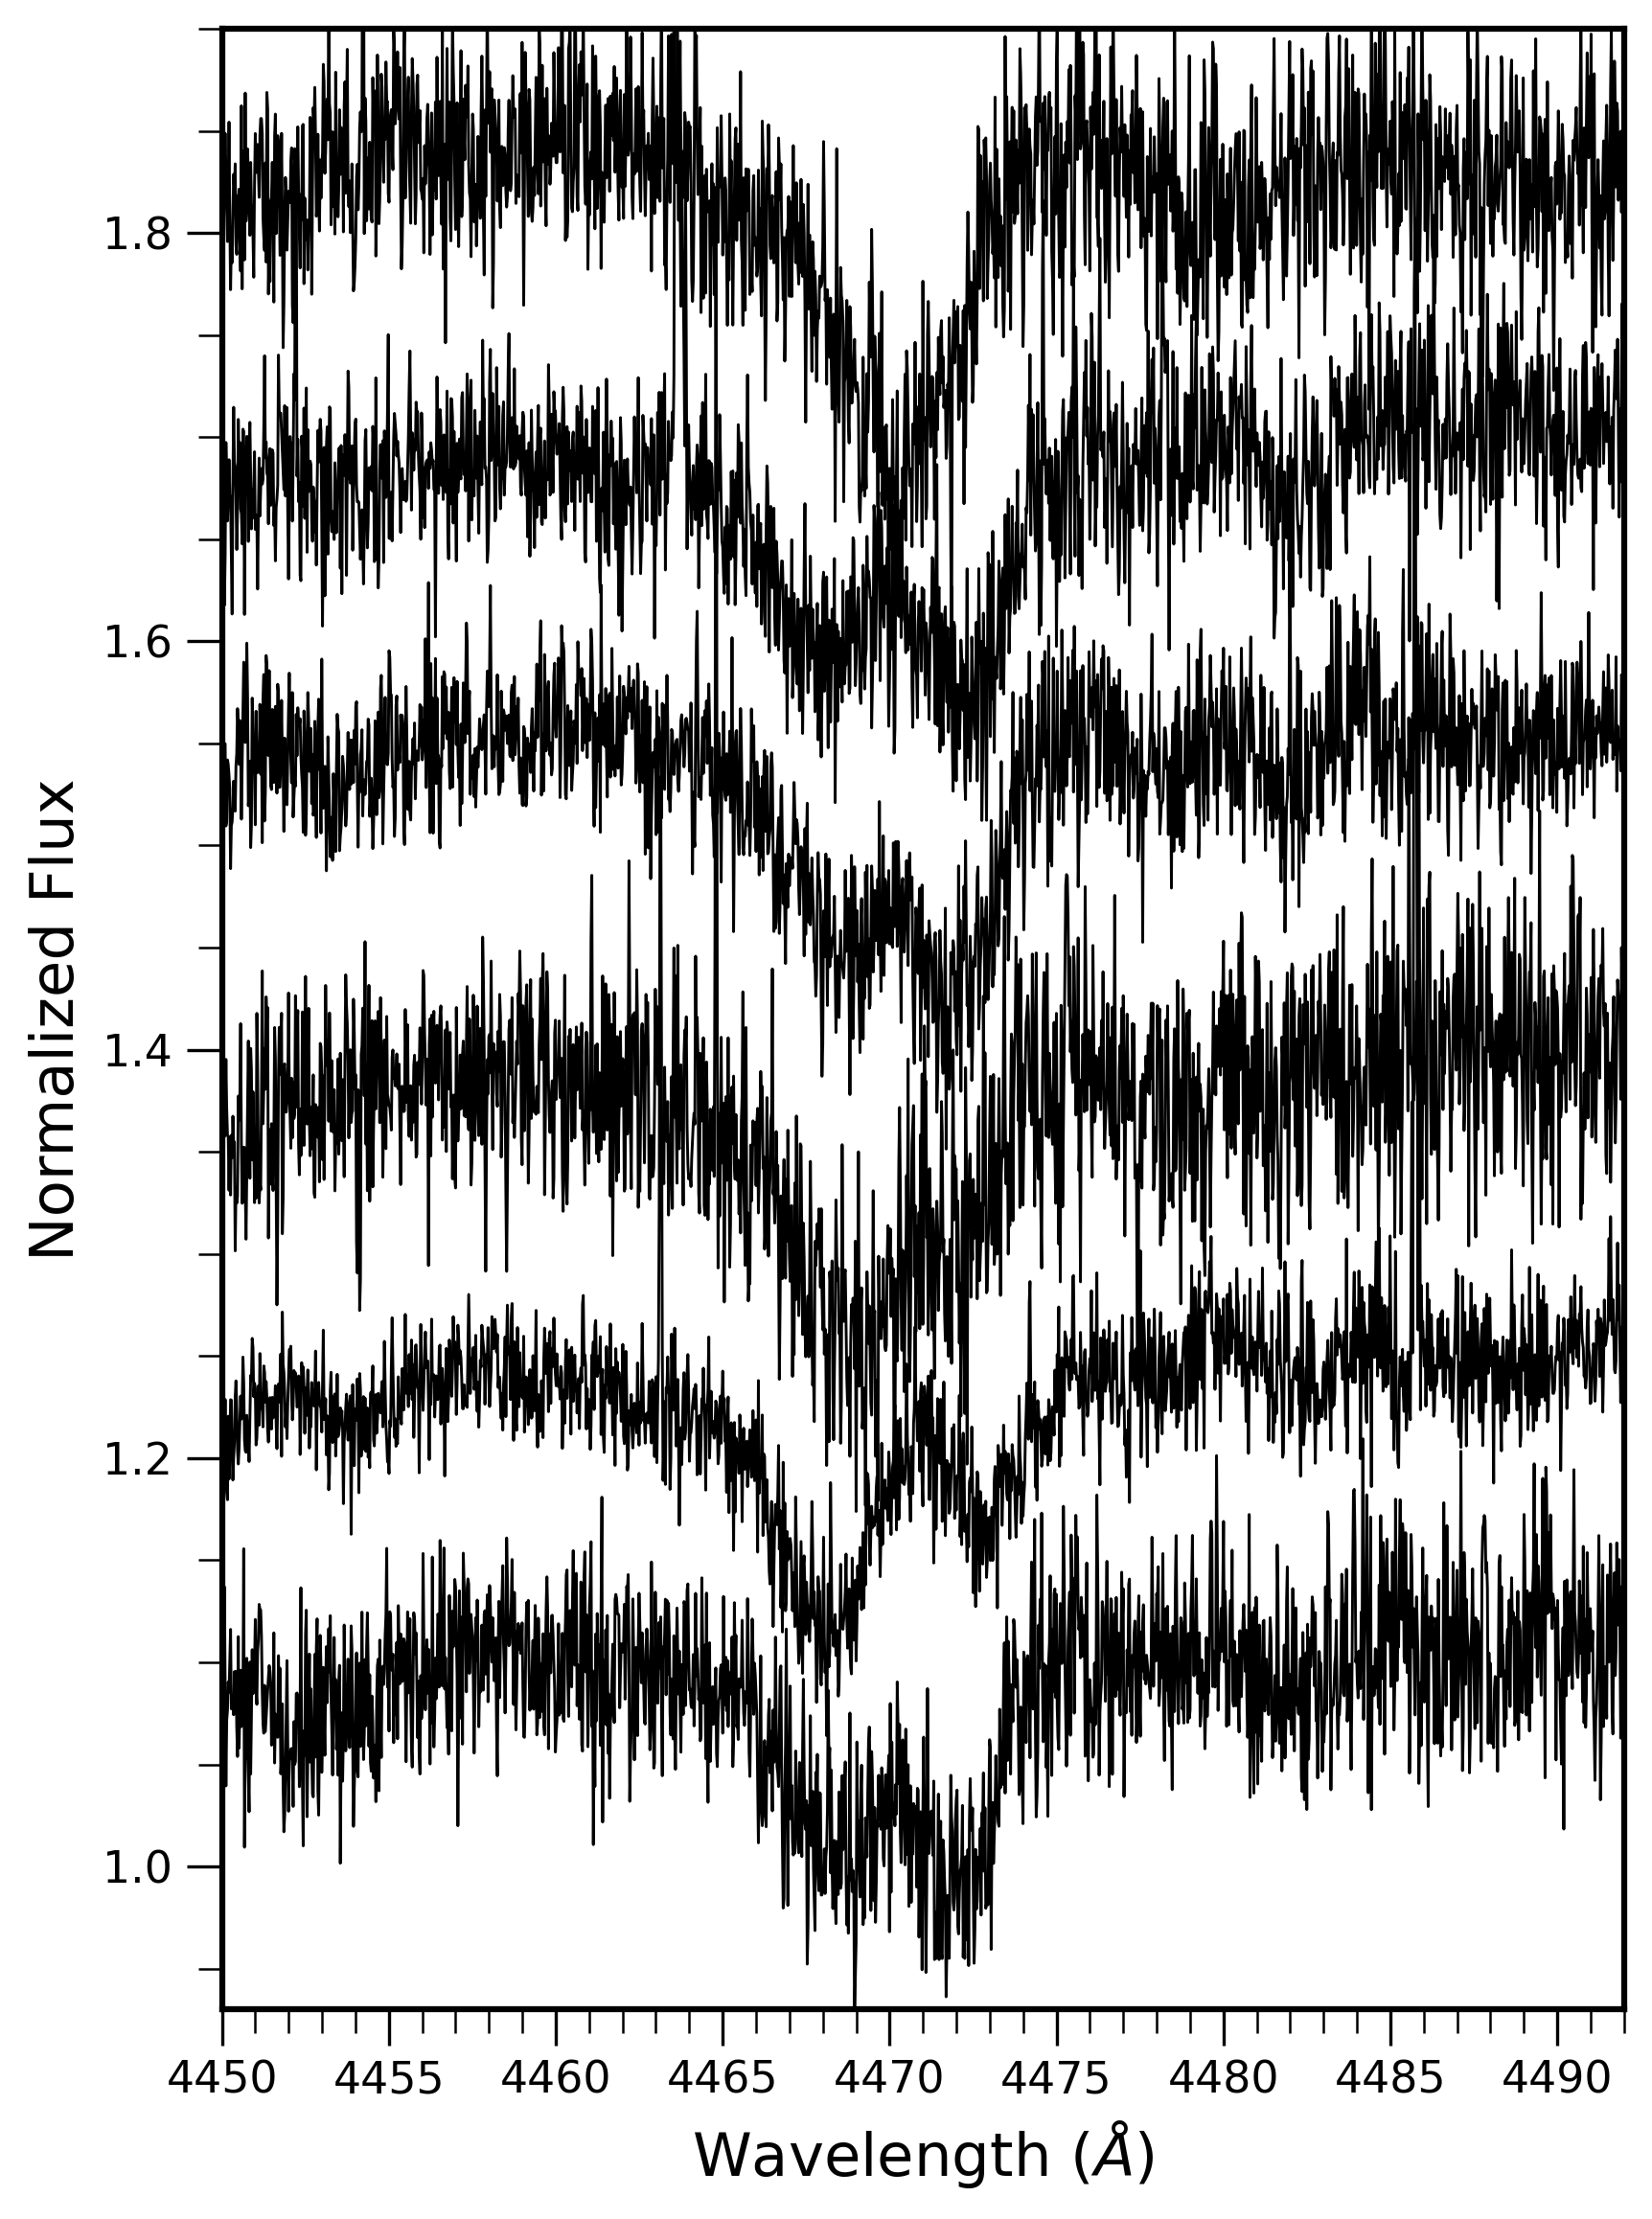
\includegraphics[width=0.7\textwidth]{chapters/WNE/image/WR157_he1_bw.png}
    \caption{He\,{\sc{i}}\,$\lambda 4471$ line for WR 157. Six epochs of spectra are stacked with an arbitrary distance apart to demonstrate its SB3 nature.}
    \label{fig:WR157_he1}
\end{figure}
\section{Relative RV measurements}\label{s:tables_RV_WNE}
Relative RVs for the objects in our sample. The reference epoch has a RV of 0.0\,\kms{}. We refrain from providing absolute RV measurements as this is highly method dependent, especially for WR stars. The Barycentric Julian Date (BJD) is given as the middle of the exposure. The average S/N is given in Table \ref{tab:wr_epochs}. Along with the measured RVs, we have indicated the measurement error, that is, the statistical uncertainty $\sigma_p$ (Eq. \ref{eq:sig_RV}). 
\begin{table}[h!]
    \centering
    \caption{Journal of HERMES observations for WR 1. Mask used: wings of the \NVred{}}
    \begin{tabular}{ccc} \hline \hline
        BJD $-$ 2450000 (d) & Relative RV (\kms) & $\sigma_p$ (\kms) \\ \hline
        7966.6224 & 12.6 & 3.5 \\ 
        8090.5018 & 5.9 & 6.6 \\ 
        8102.3783 & $-$2.5 & 3.9 \\ 
        8131.3316 & 0.0 & 2.5 \\ 
        8713.6443 & 8.6 & 3.1 \\ 
        8714.5128 & 7.4 & 2.6 \\ 
        8717.6878 & $-$6.5 & 3.7 \\ 
        8774.6470 & $-$3.1 & 4.7 \\ 
        8779.4524 & $-$24.9 & 4.6 \\ 
        8789.5124 & $-$18.2 & 6.7 \\ 
        8796.5305 & $-$7.1 & 4.0 \\ 
        8817.3615 & 3.0 & 5.9 \\ 
        8826.5518 & $-$6.6 & 5.1 \\ 
        8856.3320 & $-$11.5 & 8.4 \\ 
        8860.3339 & $-$14.5 & 4.4 \\ 
        8878.3833 & $-$14.8 & 3.4 \\ 
        9081.6208 & $-$6.3 & 3.9 \\ 
        9082.6225 & 7.1 & 3.7 \\ 
        9146.5251 & $-$4.2 & 3.4 \\ 
        9152.4444 & $-$8.3 & 4.4 \\ 
        9153.4682 & $-$7.5 & 4.5 \\ 
        9154.4621 & 3.9 & 6.0 \\ 
        9155.5839 & $-$4.4 & 6.3 \\ 
        9156.5588 & $-$15.5 & 4.7 \\ 
        9170.4167 & $-$11.1 & 5.4 \\ 
        9206.3990 & $-$9.8 & 4.2 \\ 
        9230.3722 & $-$7.8 & 6.2 \\ \hline
    \end{tabular}
    \label{tab:WR1}
\end{table}

\begin{table}[h!]
    \centering
    \caption{Journal of HERMES observations for WR 2. Mask used: full spec.}
    \begin{tabular}{ccc} \hline \hline
        BJD $-$ 2450000 (d) & Relative RV (\kms) & $\sigma_p$ (\kms) \\ \hline
        8089.4747 & 13.7 & 1.4 \\ 
        8102.3978 & $-$23.2 & 4.8 \\ 
        8131.3613 & 0.0 & 3.4 \\ 
        8739.6347 & $-$16.1 & 4.3 \\ 
        8742.6421 & $-$10.4 & 4.5 \\ 
        8744.6089 & $-$13.6 & 4.9 \\ 
        8753.6487 & $-$7.1 & 3.3 \\ 
        8774.6743 & $-$8.9 & 3.5 \\ 
        8817.4228 & $-$16.8 & 5.4 \\ 
        9081.6507 & 2.8 & 3.2 \\ 
        9089.6989 & 8.9 & 3.0 \\ 
        9146.5668 & $-$1.2 & 3.4 \\ 
        9148.4564 & $-$4.4 & 5.6 \\ 
        9170.4916 & $-$15.0 & 4.2 \\ 
        9171.3888 & $-$5.4 & 4.3 \\ 
        9172.3591 & $-$2.3 & 4.7 \\ 
        9173.4578 & $-$9.6 & 4.4 \\ 
        9174.3348 & $-$0.4 & 3.6 \\ \hline
    \end{tabular}
    \label{tab:WR2}
\end{table}

\begin{table}[h!]
    \centering
    \caption{Journal of HERMES observations for WR 3. Mask used: \NVred{}.}
    \begin{tabular}{ccc} \hline \hline
        BJD $-$ 2450000 (d) & Relative RV (\kms) & $\sigma_p$ (\kms) \\ \hline
        8786.6329 & $-$3.4 & 0.9 \\ 
        8817.4783 & 0.6 & 1.1 \\ 
        8854.4345 & 0.0 & 0.9 \\ 
        8876.3900 & 0.1 & 1.0 \\ 
        8878.4478 & 1.5 & 1.1 \\ 
        8892.3619 & 1.1 & 1.5 \\ 
        8898.3471 & $-$0.7 & 1.3 \\ 
        8906.3982 & $-$3.5 & 1.1 \\ \hline
    \end{tabular}
    \label{tab:WR3}
\end{table}

\begin{table}[h!]
    \centering
    \caption{Journal of HERMES observations for WR 6. Mask used: full spec.}
    \begin{tabular}{ccc} \hline \hline
        BJD $-$ 2450000 (d) & Relative RV (\kms{}) & $\sigma_p$ (\kms{}) \\ \hline
        8131.5571 & 2.7 & 6.0 \\ 
        8139.5854 & 3.9 & 5.5 \\ 
        8165.4858 & $-$7.9 & 10.3 \\ 
        8220.3593 & $-$55.0 & 7.9 \\ 
        8227.3515 & 62.1 & 7.0 \\ 
        8796.7597 & 14.2 & 6.7 \\ 
        8799.7682 & $-$106.0 & 6.4 \\ 
        8804.7649 & 0.0 & 5.4 \\ 
        8809.6896 & $-$83.2 & 4.5 \\ 
        8818.6700 & $-$107.9 & 3.7 \\ 
        8854.5539 & $-$67.1 & 5.1 \\ 
        8859.5353 & $-$98.4 & 4.4 \\ 
        8876.4221 & $-$50.7 & 4.4 \\ 
        8876.4272 & $-$60.1 & 4.0 \\ 
        8876.4324 & $-$48.1 & 4.2 \\ 
        8876.5373 & $-$55.3 & 4.0 \\ 
        8876.5425 & $-$55.3 & 4.2 \\ 
        8876.5477 & $-$48.8 & 4.1 \\ 
        8876.5529 & $-$52.5 & 4.4 \\ 
        8876.5581 & $-$52.9 & 4.8 \\ 
        8876.5634 & $-$58.2 & 3.7 \\ 
        9147.7394 & $-$6.6 & 7.0 \\ 
        9149.7643 & $-$0.7 & 7.3 \\ 
        9150.7615 & $-$57.9 & 6.6 \\ 
        9151.7686 & $-$2.5 & 5.9 \\ 
        9152.7737 & 0.2 & 9.6 \\ 
        9155.7095 & 4.4 & 5.8 \\ 
        9156.7172 & $-$11.3 & 6.7 \\ \hline
    \end{tabular}
    \label{tab:WR6}
\end{table}

\begin{table}[h!]
    \centering
    \caption{Journal of HERMES observations for WR 7. Mask used: \NVred.}
    \begin{tabular}{ccc} \hline \hline
        BJD $-$ 2450000 (d) & Relative RV (\kms) & $\sigma_p$ (\kms) \\ \hline
        8167.4273 & $-$11.5 & 1.2 \\ 
        8183.3812 & $-$10.4 & 1.2 \\ 
        8214.4138 & 0.0 & 1.1 \\ 
        8220.3859 & $-$20.9 & 1.1 \\ 
        8225.3718 & $-$18.4 & 1.3 \\ 
        8786.7478 & $-$25.3 & 1.5 \\ 
        8809.7142 & $-$46.5 & 1.9 \\ \hline
    \end{tabular}
    \label{tab:WR7}
\end{table}

\begin{table}[h!]
    \centering
    \caption{Journal of HERMES observations for WR 10. Mask used: full spec.}
    \begin{tabular}{ccc} \hline \hline
        BJD $-$ 2450000 (d) & Relative RV (\kms) & $\sigma_p$ (\kms) \\ \hline
        8139.6049 & 2.7 & 0.6 \\ 
        8166.4471 & 0.0 & 0.7 \\ 
        8188.4025 & $-$0.7 & 0.7 \\ 
        8223.3767 & 3.4 & 0.8 \\ 
        8226.3695 & $-$4.5 & 0.6 \\ 
        8817.7041 & 5.7 & 0.8 \\ \hline
    \end{tabular}
    \label{tab:WR10}
\end{table}

\begin{table}[h!]
    \centering
    \caption{Journal of HERMES observations for WR 110. Mask used: full spec.}
    \begin{tabular}{ccc} \hline \hline
        BJD $-$ 2450000 (d) & Relative RV (\kms) & $\sigma_p$ (\kms) \\ \hline
        7880.6775 & $-$2.4 & 2.1 \\ 
        7904.6723 & 1.9 & 2.3 \\ 
        7907.6736 & $-$9.4 & 2.8 \\ 
        8227.7273 & $-$14.1 & 3.1 \\ 
        8249.6929 & $-$20.3 & 2.2 \\ 
        8255.6409 & 4.7 & 2.8 \\ 
        8662.5573 & 0.0 & 2.8 \\ 
        8717.4911 & $-$27.1 & 5.9 \\ 
        8721.4891 & $-$19.1 & 4.3 \\ 
        9002.6274 & 4.1 & 3.4 \\ 
        9022.5824 & $-$13.7 & 2.5 \\ \hline
    \end{tabular}
    \label{tab:WR110}
\end{table}

\begin{table}[h!]
    \centering
    \caption{Journal of HERMES observations for WR 127.  Mask used: \NVred.}
    \begin{tabular}{ccc} \hline \hline
        BJD $-$ 2450000 (d) & Relative RV (\kms) & $\sigma_p$ (\kms) \\ \hline
        6383.7311 & 269.4 & 2.5 \\ 
        7925.6481 & 190.6 & 2.7 \\ 
        7958.5570 & 128.5 & 6.3 \\ 
        7965.6804 & 27.0 & 3.2 \\ 
        8262.6484 & 0.0 & 2.9 \\ 
        8317.6849 & 137.1 & 3.0 \\ 
        8624.6814 & 36.4 & 5.2 \\ 
        8669.6351 & 292.6 & 3.3 \\ 
        8677.4986 & 332.0 & 3.4 \\ 
        9001.5189 & 274.0 & 2.2 \\ 
        9029.5713 & 201.6 & 2.5 \\ \hline
    \end{tabular}
    \label{tab:WR127}
\end{table}

\begin{table}[h!]
    \centering
    \caption{Journal of HERMES observations for WR 128. Mask used: \nv{} weak.}
    \begin{tabular}{ccc} \hline \hline
        BJD $-$ 2450000 (d) & Relative RV (\kms) & $\sigma_p$ (\kms) \\ \hline
        7914.7009 & $-$3.9 & 0.8 \\ 
        7949.6014 & $-$5.4 & 1.3 \\ 
        7965.6303 & $-$6.9 & 1.1 \\ 
        7965.6540 & $-$2.6 & 1.1 \\ 
        8201.7115 & $-$9.5 & 1.0 \\ 
        8678.6017 & $-$9.7 & 1.4 \\ 
        8749.5071 & 0.0 & 1.1 \\ 
        8762.4726 & $-$4.6 & 1.6 \\ 
        9009.6923 & $-$4.1 & 0.8 \\ 
        9034.6393 & $-$4.4 & 1.3 \\ \hline
    \end{tabular}
    \label{tab:WR128}
\end{table}

\begin{table}[h!]
    \centering
    \caption{Journal of HERMES observations for WR 133. Mask used: \NVred{}.}
    \begin{tabular}{ccc} \hline \hline
        BJD $-$ 2450000 (d) & Relative RV (\kms) & $\sigma_p$ (\kms) \\ \hline
        6118.7225 & 57.5 & 3.7 \\ 
        6118.7252 & 58.1 & 4.2 \\ 
        6118.7279 & 60.1 & 3.8 \\ 
        6488.7325 & 0.0 & 1.8 \\ 
        6889.5771 & 80.7 & 2.1 \\ 
        6890.5661 & 93.8 & 2.1 \\ 
        7896.6971 & 79.1 & 3.5 \\ 
        7902.6919 & 77.7 & 3.3 \\ 
        7914.7239 & 68.8 & 3.3 \\ 
        8184.7739 & 42.7 & 4.0 \\ 
        8206.6924 & 27.4 & 4.1 \\ 
        8262.6628 & 30.1 & 2.7 \\ 
        8308.6629 & 41.2 & 4.0 \\ 
        8310.7398 & 24.0 & 4.1 \\ 
        8608.7226 & 20.2 & 3.2 \\ 
        8626.7249 & $-$17.8 & 2.8 \\ 
        8652.5782 & 20.2 & 2.6 \\ 
        8779.4212 & 59.0 & 4.7 \\ 
        8921.7629 & 80.9 & 6.3 \\ 
        8999.6873 & 48.6 & 4.0 \\ 
        9008.7106 & 44.7 & 3.1 \\ \hline
    \end{tabular}
    \label{tab:WR133}
\end{table}

\begin{table}[h!]
    \centering
    \caption{Journal of HERMES observations for WR 138. Mask used: \nv{} weak.}
    \begin{tabular}{ccc} \hline \hline
        BJD $-$ 2450000 (d) & Relative RV (\kms) & $\sigma_p$ (\kms) \\ \hline
        6126.4561 & 87.3 & 2.0 \\ 
        6126.4602 & 81.2 & 1.9 \\ 
        6126.4643 & 75.8 & 2.0 \\ 
        6890.5817 & 29.4 & 0.8 \\ 
        7902.7238 & 83.0 & 1.1 \\ 
        7938.6839 & 82.0 & 1.1 \\ 
        7966.6459 & 73.3 & 1.3 \\ 
        8199.7580 & 57.1 & 1.4 \\ 
        8209.7583 & 48.5 & 1.3 \\ 
        8265.6425 & 48.4 & 1.3 \\ 
        8309.6314 & 42.2 & 1.8 \\ 
        8629.7285 & 14.5 & 1.3 \\ 
        8705.5768 & $-$3.1 & 1.7 \\ 
        8706.6016 & 5.1 & 1.2 \\ 
        8707.5636 & 6.0 & 1.7 \\ 
        8708.5046 & $-$2.7 & 1.2 \\ 
        8709.4356 & 4.9 & 1.2 \\ 
        8710.5668 & 0.0 & 1.3 \\ 
        8712.5364 & 4.4 & 1.6 \\ 
        8713.5060 & 5.7 & 1.6 \\ 
        8714.4872 & 6.9 & 1.4 \\ 
        8715.4997 & 9.0 & 1.3 \\ 
        8716.4250 & 5.5 & 1.3 \\ 
        8716.5228 & 5.2 & 1.2 \\ 
        8716.6573 & 3.3 & 1.4 \\ 
        8717.5872 & 9.3 & 1.5 \\ 
        8718.4849 & 5.0 & 1.3 \\ 
        8719.4380 & 3.8 & 1.5 \\ 
        8720.4098 & 4.8 & 2.2 \\ 
        8721.5385 & $-$4.9 & 1.5 \\ 
        8726.4055 & 10.4 & 1.2 \\ 
        8726.4439 & 1.0 & 1.5 \\ 
        8726.4945 & 5.3 & 1.3 \\ 
        8726.5372 & 4.2 & 1.3 \\ 
        8726.5798 & 7.5 & 1.4 \\ 
        8726.6220 & 7.4 & 1.3 \\ 
        8796.4390 & 7.7 & 1.6 \\ 
        8800.3992 & 2.3 & 2.2 \\ 
        9008.7211 & 41.9 & 1.2 \\ 
        9024.5965 & 37.9 & 1.2 \\ \hline
    \end{tabular}
    \label{tab:WR138}
\end{table}

\begin{table}[h!]
    \centering
    \caption{Journal of HERMES observations for WR 139. Mask used: \NVred{}.}
    \begin{tabular}{ccc} \hline \hline
        BJD $-$ 2450000 (d) & Relative RV (\kms) & $\sigma_p$ (\kms) \\ \hline
        6126.6048 & $-$217.3 & 8.1 \\ 
        6126.6090 & $-$232.2 & 9.0 \\ 
        6126.6131 & $-$231.8 & 7.4 \\ 
        6889.3780 & $-$80.4 & 1.4 \\ 
        6889.5173 & $-$38.7 & 1.4 \\ 
        6889.6903 & 29.5 & 3.0 \\ 
        6890.3932 & 274.2 & 1.3 \\ 
        6890.5345 & 280.2 & 1.2 \\ 
        6890.6132 & 275.1 & 2.8 \\ 
        6892.4109 & $-$290.3 & 4.3 \\ 
        6892.5832 & $-$338.1 & 5.7 \\ 
        6892.6850 & $-$285.8 & 6.1 \\ 
        6894.3711 & 212.3 & 1.3 \\ 
        6894.5183 & 261.5 & 1.0 \\ 
        6894.6484 & 259.0 & 1.2 \\ 
        6896.4061 & $-$236.0 & 3.2 \\ 
        6896.5401 & $-$247.7 & 6.9 \\ 
        6896.6318 & $-$274.3 & 5.3 \\ 
        6931.5018 & $-$100.1 & 2.2 \\ 
        6946.3462 & 0.0 & 2.1 \\ 
        6946.4447 & $-$64.2 & 2.8 \\ 
        7915.7128 & $-$227.3 & 6.0 \\ 
        7919.7200 & $-$130.5 & 3.8 \\ 
        7938.6750 & 78.2 & 1.9 \\ 
        8199.7629 & 21.2 & 2.7 \\ 
        8267.5991 & 192.4 & 2.7 \\ 
        8277.7066 & $-$95.6 & 3.0 \\ 
        8277.7119 & $-$91.1 & 3.6 \\ 
        8663.7305 & 247.9 & 1.9 \\ 
        8682.5103 & $-$243.0 & 5.7 \\ 
        8741.4968 & $-$250.7 & 5.2 \\ 
        8779.4428 & $-$281.8 & 11.3 \\ 
        9024.6078 & $-$255.7 & 8.2 \\ 
        9080.5344 & 167.5 & 2.2 \\ \hline
    \end{tabular}
    \label{tab:WR139}
\end{table}

\begin{table}[h!]
    \centering
    \caption{Journal of HERMES observations for WR 141. Mask used: \NVred.}
    \begin{tabular}{ccc} \hline \hline
        BJD $-$ 2450000 (d) & Relative RV (\kms) & $\sigma_p$ (\kms) \\ \hline
        6889.6476 & 74.8 & 5.1 \\ 
        6889.6690 & 47.7 & 7.9 \\ 
        7949.5642 & $-$11.9 & 4.8 \\ 
        7957.6105 & 126.0 & 4.3 \\ 
        7961.6127 & 59.2 & 4.6 \\ 
        8196.7557 & 188.7 & 3.0 \\ 
        8267.6131 & 0.0 & 2.7 \\ 
        8332.7166 & 14.9 & 2.9 \\ 
        8666.7123 & 46.6 & 3.4 \\ 
        8749.5352 & $-$15.0 & 3.0 \\ 
        8759.4257 & 152.6 & 4.4 \\ 
        8799.4244 & 136.5 & 7.4 \\ 
        9021.7199 & 146.7 & 6.8 \\ 
        9029.7067 & $-$21.1 & 6.9 \\ \hline
    \end{tabular}
    \label{tab:WR141}
\end{table}

\begin{table}[h!]
    \centering
    \caption{Journal of HERMES observations for WR 151. Mask used: \NVred.}
    \begin{tabular}{ccc} \hline \hline
        BJD $-$ 2450000 (d) & Relative RV (\kms) & $\sigma_p$ (\kms) \\ \hline
        8133.3587 & 0.0 & 9.5 \\ 
        8718.5857 & 124.8 & 19.3 \\ 
        8763.4920 & 351.8 & 31.2 \\ 
        9042.5982 & 650.0 & 41.3 \\ 
        9051.6960 & 277.9 & 15.9 \\ 
        9057.6630 & 622.4 & 34.0 \\ \hline
    \end{tabular}
    \label{tab:WR151}
\end{table}

\begin{table}[h!]
    \centering
    \caption{Journal of HERMES observations for WR 152. Mask used: \NVred.}
    \begin{tabular}{ccc} \hline \hline
        BJD $-$ 2450000 (d) & Relative RV (\kms) & $\sigma_p$ (\kms) \\ \hline
        8137.3704 & 0.0 & 1.2 \\ 
        8712.5811 & 4.7 & 1.5 \\ 
        8753.5905 & $-$0.0 & 1.6 \\ 
        8775.5911 & $-$3.0 & 1.5 \\ 
        8791.4069 & $-$2.0 & 1.3 \\ 
        9052.7004 & $-$3.6 & 1.7 \\ 
        9058.6666 & $-$0.6 & 1.5 \\ \hline
    \end{tabular}
    \label{tab:WR152}
\end{table}

\begin{table}[h!]
    \centering
    \caption{Journal of HERMES observations for WR 157. Mask used: \NVblue{}.}
    \begin{tabular}{ccc} \hline \hline
        BJD $-$ 2450000 (d) & Relative RV (\kms) & $\sigma_p$ (\kms) \\ \hline
        6890.6373 & $-$1.3 & 1.5 \\ 
        6890.6588 & $-$1.9 & 1.4 \\ 
        8091.4134 & 0.0 & 1.1 \\ 
        8321.7169 & $-$3.3 & 1.8 \\ 
        8336.6816 & $-$8.1 & 1.4 \\ 
        8665.6904 & $-$6.4 & 1.6 \\ 
        8754.5808 & $-$8.7 & 1.6 \\ 
        8762.5811 & $-$4.2 & 1.4 \\ 
        8775.4222 & 0.1 & 1.3 \\ 
        8787.4261 & 3.1 & 2.6 \\ 
        9041.7175 & $-$0.1 & 1.2 \\ 
        9058.7028 & $-$1.1 & 1.6 \\ \hline
    \end{tabular}
    \label{tab:WR157}
\end{table}


\section{Posterior plots from MC simulations}\label{s:posteriors}

Here we present the three-dimensional likelihood plots for the Bayesian analysis of the WNE sample with the assumptions and setup as described in \ref{sect:bayesian} while exploring values for the mass-ratio index ($\kappa$) of $+1.0$ (Fig. \ref{fig:kappa_plus1}) and $-1.0$ (Fig. \ref{fig:kappa_minus1}). The conclusions do not vary significantly as compared to a flat mass ratio ($\kappa=0.0$, Fig. \ref{fig:flat_pdist_binfrac}). 

\begin{figure}
    \centering
    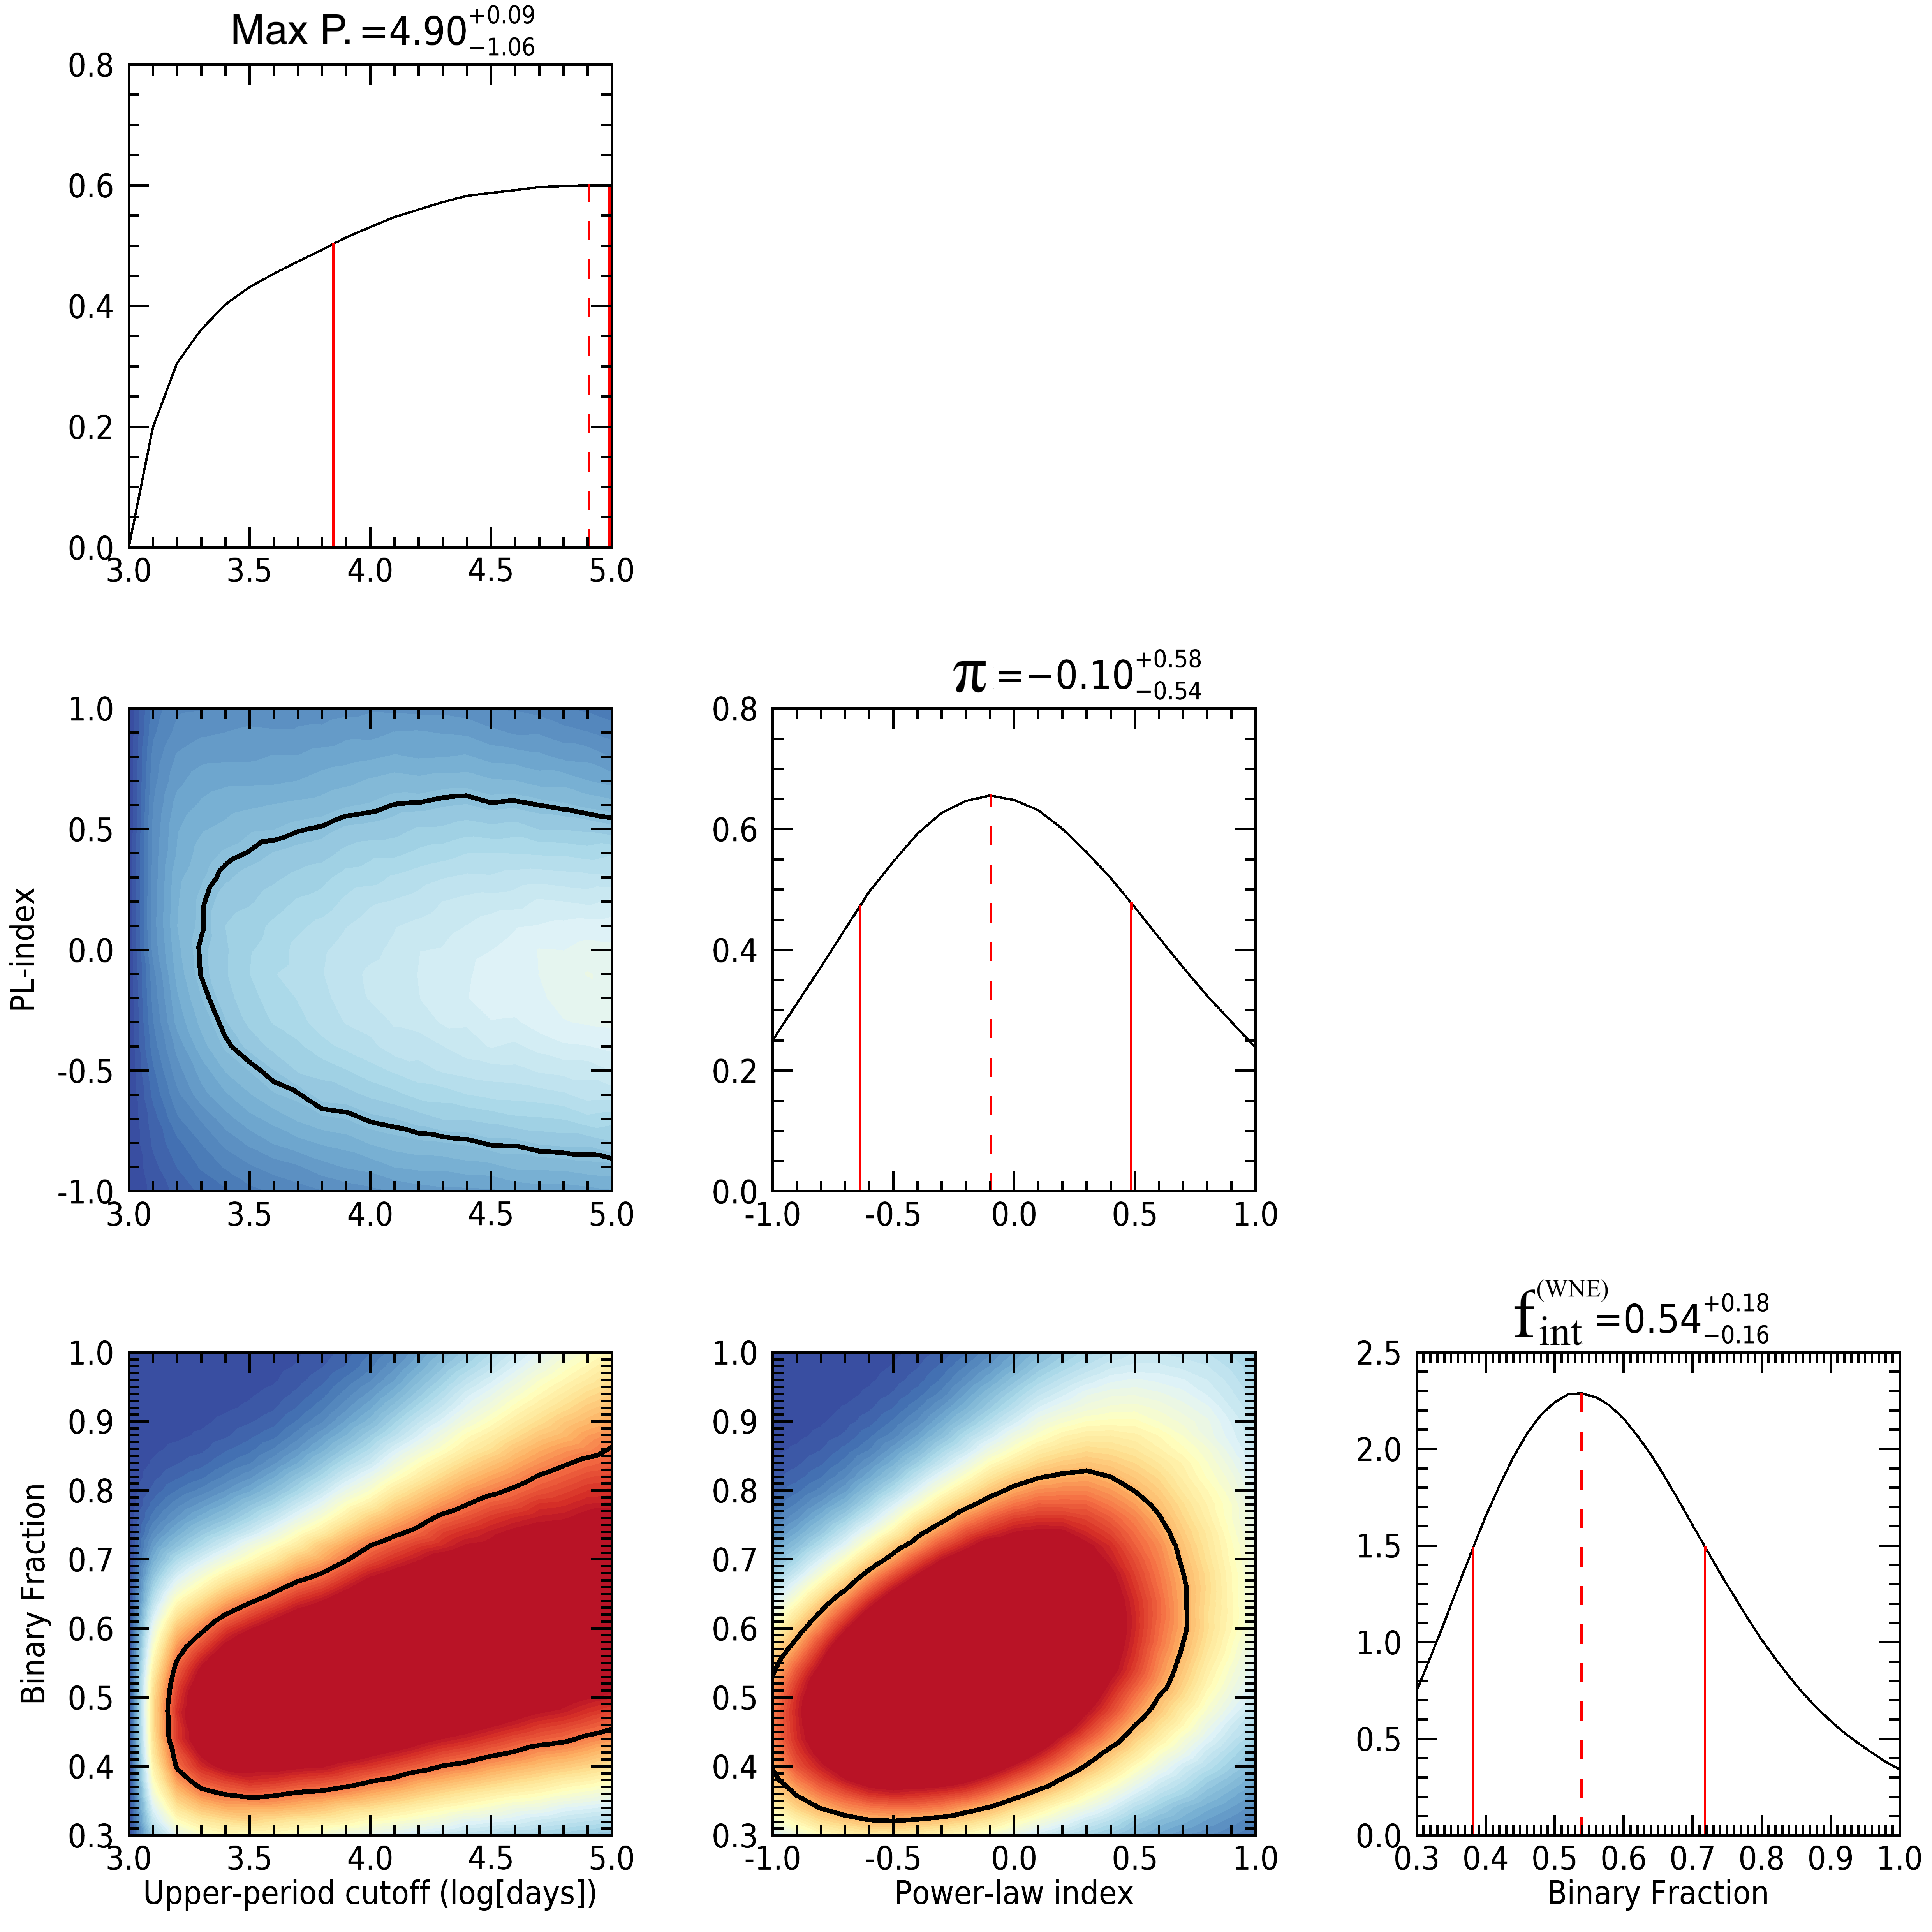
\includegraphics[width=\hsize]{chapters/WNE/image/Kappa_plus1.png}
    \caption{Posteriors for \logPmax{}, \fintWNE{} , and $\pi$ for $\kappa = +1.0$. For each posterior, the solid red lines show HDI68, and the dashed red line shows the mode.}
    \label{fig:kappa_plus1}
\end{figure}


\begin{figure}
    \centering
    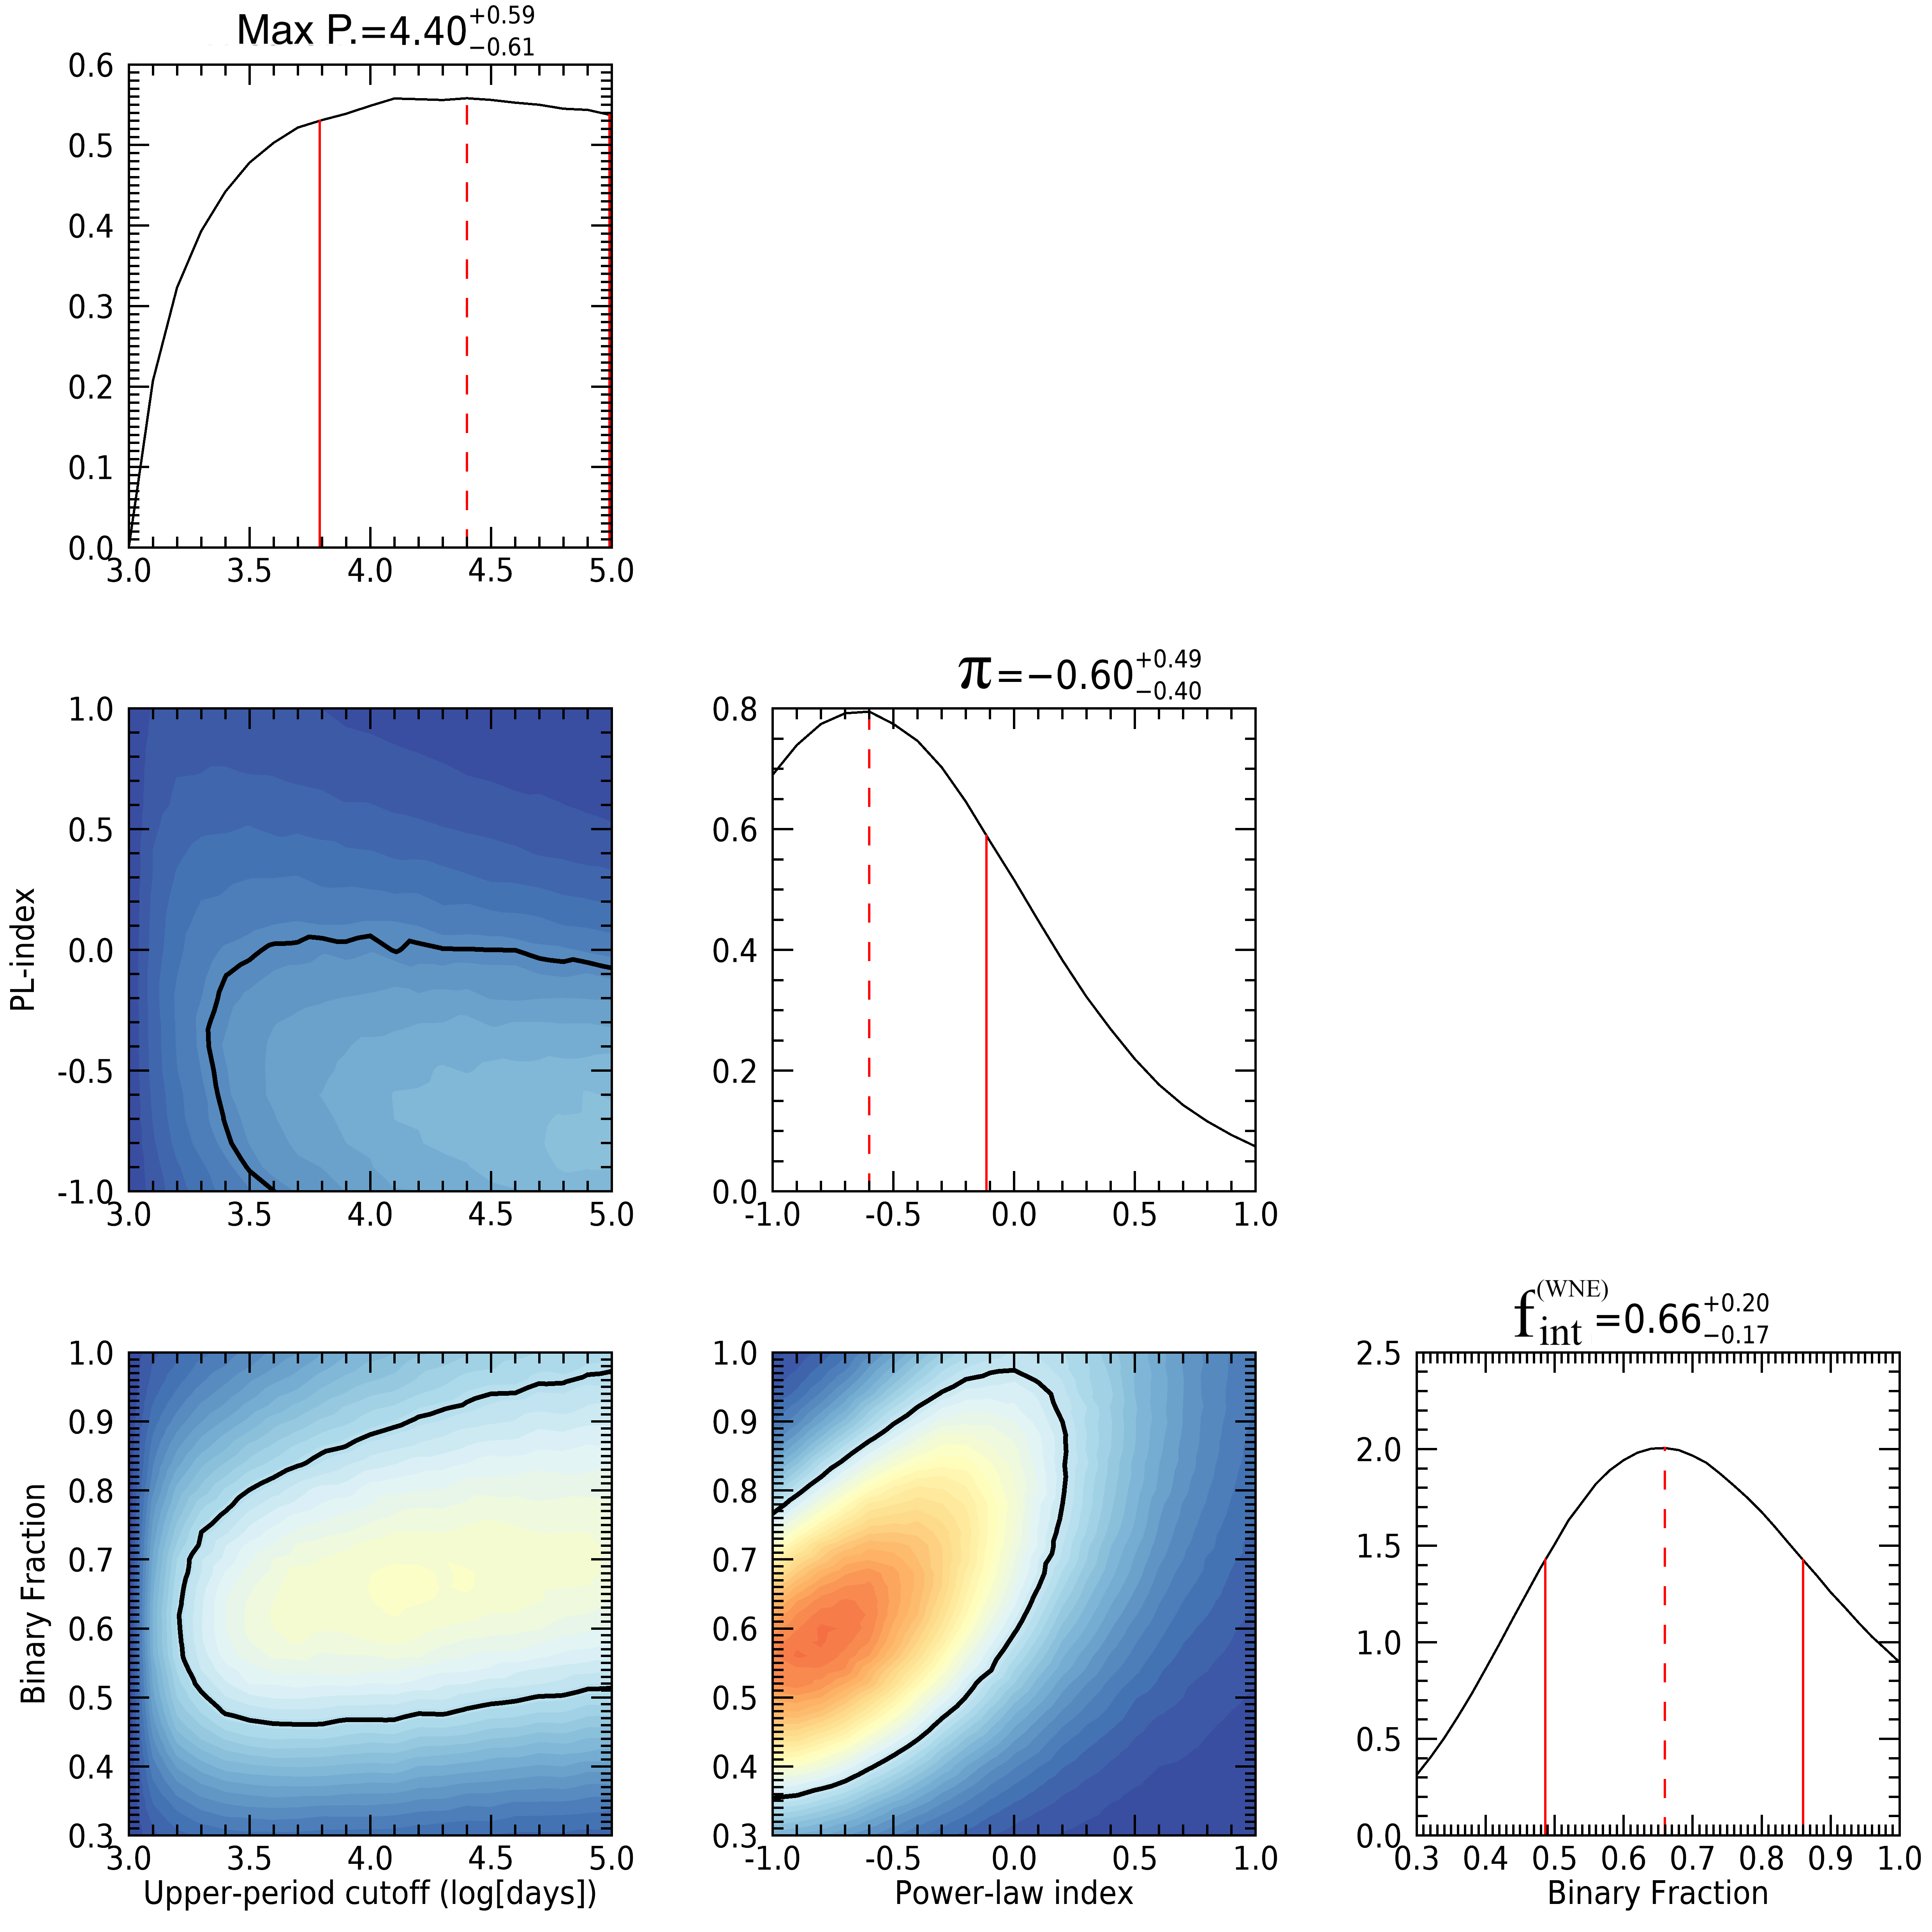
\includegraphics[width=\hsize]{chapters/WNE/image/Kappa_minus1.png}
    \caption{Posteriors for \logPmax{}, \fintWNE{} , and $\pi$ for $\kappa = -1.0$. For each posterior, the solid red lines show HDI68, and the dashed red line shows the mode.}
    \label{fig:kappa_minus1}
\end{figure}

\subsection{WC sample}
As discussed in Sect. \ref{sect:WC_bayesian}, we performed MC simulations with a Bayesian framework for the 12 Galactic WC stars in Chapter \ref{ch:wc} over four parameters, \logPmin{}, \logPmax{}, \fintWNE{} , and $\pi$ , with the same step size as for the WNE sample and over the ranges displayed in Fig.~\ref{fig:WC_posteriors}. We calculated the four-dimensional likelihood and corresponding posteriors, assuming flat priors. With this, we enable a consistent comparison of the corresponding WC and WNE populations from an evolutionary perspective.

As in Chapter \ref{ch:wc}, we divided the stars into four \DelRV{} bins: 5\,$\le$\,\DelRV{}\,$\le$\,30\,\kms{} (six targets), 30\,$\le$\,\DelRV{}\,$\le$\,250\,\kms{} (no observations), 250\,$<$\,\DelRV{}\,$\le$\,300\,\kms{} (one observation), and  \DelRV{}\,$\ge$\,300\,\kms{} (no observations). We also enforced that our simulations have binaries in the following period bins: $P > 20$\,d (three systems), $P > 2000$\,d (two systems). With this setup, we simulated 10\,000 sets of 12 WC stars for each bin in this four-dimensional parameter space, hence $\sim 7\time10^9$ populations. 
